\section{File System Interface}
\label{sec:software}

The primary design goal of the FlashBoost file system layer is to provide an
easy-to-use interface between user-level applications and hardware accelerators
in the storage device, by hiding many of the complex physical properties of
flash storage. Since NAND flash has very different characteristics from
traditional hard disk drives, a flash-aware management layer like a Flash
Translation Layer (FTL)~\cite{} is required to hide such differences from the
rest of the system.

Because conventional file systems also incorporate a translation layer to deal
with garbage collection and to optimize storage access patterns for disks, there
is a dual layer of translation, making the stack inefficient. Some file systems
have tried to remedy this by refactoring the I/O architecture in order to
offload most of the FTL functions into a flash-optimized log-structured file
system. A prominent example of this is RFS~\cite{rfs}. 
Unlike conventional FTL designs where the flash characteristics are
hidden from the file system, RFS performs some functionality of an FTL,
including logical-to-physical address mapping and garbage collection.
This helps achieve achieving better garbage collection
efficiency at much lower memory requirement. 
The file system interface in FlashBoost is built on the same paradigms, with
additional functions for in-storage processor access.

For the sake of compatibility with existing software, FlashBoost also offers a
full-fledged page-level FTL for end-users. This is is implemented in the device
driver, much like Fusion IO’s driver implementation. It allows us to use
well-known Linux file systems (e.g., ext2/4/3) as well as database systems
(directly running on top of a block device) with FlashBoost.

The FlashBoost software allows developers to easily make use of fast in-storage
processing without any efforts to write their own custom interfaces manually.
Figure~\ref{fig:filesystem} shows how user-level applications access hardware
accelerators.  In the FlashBoost software stack, user-level applications can
query the file system for the physical locations of files on the flash (see (1)
in Figure~\ref{fig:filesystem}). This was made possible because the file system
maintains the mapping information.  Applications can then provide in-storage
processors with a stream of physical addresses(see (2))
, so that the in-storage processors can directly read
data from flash with very low latency (see (3)).
The results are sent to software memory and the user application can be notified
(see (4)).

It is worth noting that, in FlashBoost, all the user requests, including both
user queries and data, are sent to the hardware directly, bypassing almost all
OS kernel, except for essential driver modules.  This helps us to avoid deep OS
kernel stacks that often cause long I/O latencies.  It is also very common that
multiple user-applications compete for the limited and precious hardware
acceleration units. For efficient sharing of hardware resources, FlashBoost runs
a scheduler that assigns available hardware-acceleration units to competing
user-applications. In our implementation, a simple FIFO-based policy is used for
request scheduling.

\begin{figure}[h]
	\begin{center}
	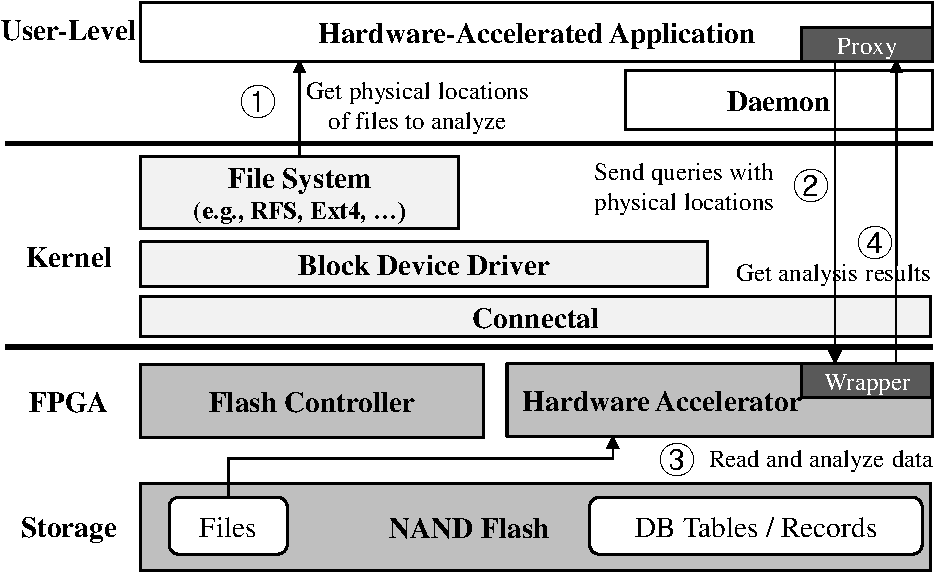
\includegraphics[width=0.4\paperwidth]{figures/software.pdf}
	\caption{File System Interface}
	\label{fig:filesystem}
	\end{center}
\end{figure}
